\documentclass[11pt]{article}
\usepackage[a4paper,margin=22mm,headheight=15pt]{geometry}
\usepackage{amsmath,amssymb,graphicx,booktabs,array,xcolor,fancyhdr,enumitem,hyperref}
\usepackage{mathptmx}
\definecolor{accent}{HTML}{176578}
\hypersetup{colorlinks=true,linkcolor=accent,urlcolor=accent}
\pagestyle{fancy}\fancyhf{}\lhead{FlowMLLab | AI in Fluids}\rhead{Week 1: Numerical foundations}\cfoot{\thepage}
\setlength{\parindent}{0pt}\setlength{\parskip}{7pt}
\setlist{nosep,leftmargin=*}
\newcommand{\topic}[2]{\section*{#1\quad #2}\addcontentsline{toc}{section}{#1: #2}}
\newcommand{\checkpoint}[1]{\par\smallskip\noindent\textcolor{accent}{\textbf{Check your understanding.}} #1\par}
\newcommand{\dd}{\mathrm{d}}
\begin{document}
\begin{center}
{\color{accent}\LARGE\bfseries AI in Fluids: Week 1}\\[8pt]
{\Large From conservation laws to a cavity solver}\\[6pt]
{\large Numerical foundations for students new to CFD}
\end{center}
\vspace{8pt}
\textbf{The learning question.} How can a computer predict the recirculating flow in a box when only the wall motion, fluid properties, and geometry are given?

A neural network can fit a field without ensuring that it conserves mass or satisfies a wall condition. This week establishes the physical and numerical language needed to judge both CFD solutions and later machine-learning predictions. We start with conservation of mass and momentum, derive a pressure-free formulation for two-dimensional incompressible flow, and connect each equation to the existing cavity notebook.

\textbf{Three companion notebooks}
\begin{enumerate}
\item \texttt{01\_python\_for\_cfd\_ai\_fluids.ipynb}: variables, functions, arrays, derivatives, and residuals.
\item \texttt{02\_tensorflow\_for\_ai\_fluids.ipynb}: tensors, shapes, losses, automatic differentiation, and a small neural network.
\item \texttt{03\_cavity\_ghia.ipynb}: a finite-difference streamfunction--vorticity solver and centerline comparison at $Re=100$.
\end{enumerate}
All three are in \texttt{notebooks/week01/}. This lecture explains the introductory $Re=100$ solver; retained pressure-validation demonstrations elsewhere in the notebook have their own conditions and evidence.

\textbf{Reading route}
\begin{center}\begin{tabular}{p{.16\linewidth}p{.75\linewidth}}
\toprule
Pages & Topic\\\midrule
2--3 & Fluid fields; continuity and both momentum components\\
4 & Deriving the nondimensional equations and $1/Re$\\
5--7 & Streamfunction, vorticity, proof of original Eq.~(15), optional transport derivation\\
8--9 & Finite differences and wall boundary conditions\\
10--11 & Coupled iteration, convergence, and stability\\
12--13 & Benchmarks, optional pressure recovery, and assessment\\\bottomrule
\end{tabular}\end{center}
\textbf{Conventions.} A right-handed $(x,y,z)$ system is used, with $x$ rightward and $y$ upward. Positive $\omega=\omega_z$ means counterclockwise local rotation. Dimensional quantities have a subscript $d$ when scales are introduced. After nondimensionalization, unadorned variables are dimensionless.

\textbf{Scope.} A constant-density, constant-viscosity Newtonian fluid; two-dimensional incompressible motion; no nonconservative body force. The cavity is a square with a uniformly translating top wall. This is a teaching model, not a model for rarefied or compressible flow.
\newpage
\topic{1}{Fluids, fields, and acceleration}
A fluid continuously deforms under an applied shear stress. Both liquids and gases are fluids. In the continuum description, density, velocity, pressure, and temperature are fields rather than properties of individually tracked molecules. The approximation requires molecular length scales to be small compared with the relevant flow scales.

\begin{center}\begin{tabular}{lll}\toprule
Symbol & Meaning & SI unit\\\midrule
$\rho$ & Density & $\mathrm{kg\,m^{-3}}$\\
$\boldsymbol{u}_d=(u_d,v_d)$ & Velocity & $\mathrm{m\,s^{-1}}$\\
$p_d$ & Pressure & $\mathrm{Pa}$\\
$\mu$ & Dynamic viscosity & $\mathrm{Pa\,s}$\\
$\nu=\mu/\rho$ & Kinematic viscosity & $\mathrm{m^2\,s^{-1}}$\\
$\psi_d$ & Two-dimensional streamfunction & $\mathrm{m^2\,s^{-1}}$\\
$\omega_d$ & Out-of-plane vorticity & $\mathrm{s^{-1}}$\\\bottomrule
\end{tabular}\end{center}
In an Eulerian description, $u_d=u_d(x_d,y_d,t_d)$: we ask what passes a fixed position. A Lagrangian description instead follows a moving particle. The cavity notebook uses Eulerian arrays, with \texttt{u[j,i]} representing the horizontal velocity at $(x_i,y_j)$.

\textbf{Why acceleration is not just a time derivative.} Follow a fluid particle with $\dd x_d/\dd t_d=u_d$ and $\dd y_d/\dd t_d=v_d$. Applying the chain rule to its horizontal velocity gives
\begin{equation}
\frac{D u_d}{D t_d}=\frac{\partial u_d}{\partial t_d}+u_d\frac{\partial u_d}{\partial x_d}+v_d\frac{\partial u_d}{\partial y_d}.
\end{equation}
The first term describes change at a fixed point; the last two describe change as the particle moves through a nonuniform field. A steady flow can therefore have nonzero acceleration. The vector statement is
\begin{equation}
\frac{D\boldsymbol{u}_d}{Dt_d}=\frac{\partial\boldsymbol{u}_d}{\partial t_d}+(\boldsymbol{u}_d\cdot\nabla_d)\boldsymbol{u}_d.
\end{equation}
\textbf{From physics to arrays}
\begin{itemize}
\item A continuous field becomes values at grid nodes, not a photograph of exact values everywhere.
\item A spatial derivative becomes a difference between neighboring entries.
\item Boundary conditions become constraints on boundary entries.
\item A residual measures an equation defect or an iteration change; neither is automatically the error relative to the exact solution.
\end{itemize}
\checkpoint{Can a particle accelerate when $\partial\boldsymbol{u}_d/\partial t_d=0$? Explain using a particle turning around a cavity vortex.}
\newpage
\topic{2}{Review: continuity and momentum}
\textbf{Mass conservation.} The general continuity equation is
\begin{equation}
\frac{\partial\rho}{\partial t_d}+\nabla_d\cdot(\rho\boldsymbol{u}_d)=0.
\end{equation}
For the constant-density fluid used here, it becomes
\begin{equation}\boxed{\frac{\partial u_d}{\partial x_d}+\frac{\partial v_d}{\partial y_d}=0.}\label{eq:mass}\end{equation}
A small material fluid element preserves its volume: local inflow and outflow balance. This does not require either velocity component to be spatially constant.

\textbf{Momentum conservation.} For an incompressible Newtonian fluid with constant properties and no body force, the two component equations are
\begin{align}
\underbrace{\frac{\partial u_d}{\partial t_d}}_{\text{local change}}+
\underbrace{u_d\frac{\partial u_d}{\partial x_d}+v_d\frac{\partial u_d}{\partial y_d}}_{\text{convection}}
&=\underbrace{-\frac{1}{\rho}\frac{\partial p_d}{\partial x_d}}_{\text{pressure force}}+
\underbrace{\nu\left(\frac{\partial^2u_d}{\partial x_d^2}+\frac{\partial^2u_d}{\partial y_d^2}\right)}_{\text{viscous diffusion}},\label{eq:xmom}\\
\frac{\partial v_d}{\partial t_d}+u_d\frac{\partial v_d}{\partial x_d}+v_d\frac{\partial v_d}{\partial y_d}
&=-\frac{1}{\rho}\frac{\partial p_d}{\partial y_d}+\nu\left(\frac{\partial^2v_d}{\partial x_d^2}+\frac{\partial^2v_d}{\partial y_d^2}\right).\label{eq:ymom}
\end{align}
Every term has units of acceleration. Pressure gradients push fluid from high toward low pressure; viscosity diffuses momentum between neighboring regions. Convection is nonlinear because the unknown velocity multiplies derivatives of the unknown velocity.

\textbf{Three unknown fields.} Equations~\eqref{eq:mass}--\eqref{eq:ymom} couple $u_d$, $v_d$, and $p_d$. Pressure-based CFD algorithms can solve this system directly while enforcing incompressibility. In this lecture we transform it into a system for $\psi$ and $\omega$ that is especially convenient for a two-dimensional simply connected cavity. The transformed system still represents momentum conservation.

\textbf{Initial and boundary data.} A time-dependent problem also needs an initial velocity field consistent with incompressibility and the prescribed conditions. The teaching solver starts from zero interior fields and applies the moving lid impulsively. The initial boundary jump creates a transient before the flow approaches a steady state.

\checkpoint{Write the vertical convective acceleration. Why would using only the horizontal momentum equation leave the cavity problem incomplete?}
\newpage
\topic{3}{Deriving the nondimensional equations}
Let $L$ be the cavity side length and $U>0$ the lid-speed scale. Choose the convective time $L/U$ and dynamic pressure $\rho U^2$. Define
\begin{equation}
x=\frac{x_d}{L},\quad y=\frac{y_d}{L},\quad t=\frac{t_dU}{L},\quad
u=\frac{u_d}{U},\quad v=\frac{v_d}{U},\quad p=\frac{p_d-p_{\rm ref}}{\rho U^2}.
\end{equation}
All variables in these ratios are now dimensionless. The chain rule gives, for example,
\[
\frac{\partial u_d}{\partial t_d}=\frac{U^2}{L}u_t,\qquad
u_d\frac{\partial u_d}{\partial x_d}=\frac{U^2}{L}u u_x,
\]
\[
\frac{1}{\rho}(p_d)_{x_d}=\frac{U^2}{L}p_x,\qquad
\nu\nabla_d^2u_d=\frac{\nu U}{L^2}\nabla^2u.
\]
Divide horizontal momentum by $U^2/L$. The coefficient of diffusion is $\nu/(UL)=1/Re$, where
\begin{equation}\boxed{Re=\frac{UL}{\nu}=\frac{\rho UL}{\mu}.}\end{equation}
The dimensionless system, with subscripts denoting derivatives, is
\begin{align}
u_x+v_y&=0,\\
u_t+uu_x+vu_y&=-p_x+\frac{1}{Re}(u_{xx}+u_{yy}),\\
v_t+uv_x+vv_y&=-p_y+\frac{1}{Re}(v_{xx}+v_{yy}).
\end{align}
\textbf{Interpretation.} Reynolds number compares inertial and viscous effects using the chosen scales. Its value alone does not give a universal transition threshold: geometry, disturbances, and boundary conditions also matter.

\textbf{Notebook translation.} The square becomes $0\leq x,y\leq1$, and the lid speed is $u=1$. At $Re=100$, the dimensionless diffusion coefficient is $0.01$. This does \emph{not} imply a physical kinematic viscosity of $0.01\,\mathrm{m^2/s}$ unless the dimensional scales make that true. For example, $L=0.1\,\mathrm{m}$ and $U=0.01\,\mathrm{m/s}$ give $\nu=10^{-5}\,\mathrm{m^2/s}$ at the same Reynolds number.

\textbf{Two more scales.} Set $\psi=\psi_d/(UL)$ and $\omega=\omega_d L/U$. These choices preserve $u=\psi_y$, $v=-\psi_x$, and $\omega=v_x-u_y$. All equations on the following pages use dimensionless variables unless stated otherwise.
\checkpoint{Which time in seconds corresponds to dimensionless $t=10$ for the example above? Answer: $100\,\mathrm{s}$.}
\newpage
\topic{4}{Streamfunction and vorticity: definitions}
For a sufficiently smooth, two-dimensional incompressible velocity field in this simply connected domain, introduce a scalar streamfunction $\psi$ through
\begin{equation}\boxed{u=\psi_y,\qquad v=-\psi_x.}\label{eq:psi}\end{equation}
Substitution into continuity gives
\begin{equation}u_x+v_y=\psi_{yx}-\psi_{xy}=0,\end{equation}
because the mixed derivatives commute. Thus the streamfunction representation builds mass conservation into the continuous equations.

\textbf{Why its contours are streamlines.} At a fixed instant,
\begin{equation}\boldsymbol{u}\cdot\nabla\psi=u\psi_x+v\psi_y=\psi_y\psi_x-\psi_x\psi_y=0.\end{equation}
Velocity is tangent to a contour $\psi=\text{constant}$. For unsteady flow these instantaneous streamlines need not be particle paths. At fixed $x$, the volume flow rate per unit depth between $y_1$ and $y_2$ is $\int_{y_1}^{y_2}u\,\dd y=\psi(x,y_2)-\psi(x,y_1)$.

\textbf{Vorticity.} The curl of velocity has only a $z$ component in this two-dimensional flow:
\begin{equation}\boxed{\omega=v_x-u_y.}\label{eq:omega}\end{equation}
Vorticity measures local rotation; the local rigid-body angular velocity is $\omega/2$. It is not speed, and it is not the curvature of a streamline. A shear flow can have nonzero vorticity even with straight streamlines.

\textbf{Example: Couette shear.} For $u=y$, $v=0$, choose $\psi=y^2/2$. Then $u=\psi_y$, $v=-\psi_x$, and $\omega=-1$. Horizontal layers move at different speeds, producing clockwise local rotation. This sign convention is also consistent with the negative wall vorticity generated by a rightward-moving cavity lid.

\textbf{A useful numerical distinction.} Central differences for $u= D_y\psi$ and $v=-D_x\psi$ give a zero discrete divergence wherever the same commuting stencils are used. Overwriting wall velocities or switching stencils near boundaries requires separate checks; the continuum identity is not a guarantee that every boundary discretization is consistent.
\checkpoint{For solid-body rotation $u=-\Omega y$, $v=\Omega x$, find $\omega$ and a compatible $\psi$. Answer: $2\Omega$ and $-\Omega(x^2+y^2)/2$ plus a constant.}
\newpage
\topic{5}{Proof of the streamfunction Poisson equation}
\textbf{This is the proof requested for Eq.~(15) in the previous lecture.} Begin with the definitions; no new physical assumption is needed beyond those already stated:
\begin{align}
\omega&=\frac{\partial v}{\partial x}-\frac{\partial u}{\partial y},\\
v=-\psi_x&\quad\Longrightarrow\quad v_x=-\psi_{xx},\\
u=\psi_y&\quad\Longrightarrow\quad u_y=\psi_{yy}.
\end{align}
Therefore
\begin{equation}\omega=-\psi_{xx}-\psi_{yy}=-\nabla^2\psi,\end{equation}
and hence
\begin{equation}\boxed{\nabla^2\psi=-\omega.}\label{eq:poisson}\end{equation}
The minus sign follows from the paired conventions $u=\psi_y$, $v=-\psi_x$ and $\omega=v_x-u_y$. Changing only one convention would change the problem incorrectly.

\textbf{What this equation does.} If $\omega$ is known throughout the interior and appropriate wall values of $\psi$ are prescribed, Eq.~\eqref{eq:poisson} is an elliptic Poisson problem for $\psi$. Differentiating its solution then gives velocity. This is a spatial solve at each stage of the algorithm; the equation itself contains no time derivative.

\textbf{A manufactured check.} Let
\begin{equation}\psi=\sin(\pi x)\sin(\pi y).
\end{equation}
Then
\begin{align}
u&=\pi\sin(\pi x)\cos(\pi y),&
v&=-\pi\cos(\pi x)\sin(\pi y),\\
\omega&=2\pi^2\sin(\pi x)\sin(\pi y),&
\nabla^2\psi&=-2\pi^2\sin(\pi x)\sin(\pi y).
\end{align}
This verifies the sign and provides smooth fields for checking derivative code. It is a manufactured identity check, \emph{not} a no-slip cavity solution: although $\psi=0$ on the boundary, tangential velocities generally do not vanish there.

\textbf{Why $\psi=0$ on the cavity walls?} Impermeability makes $\psi$ constant along each wall. The connected cavity boundary permits one common constant; choose zero because adding a constant leaves velocity unchanged. Tangential no-slip is additional information, enforced through the wall-vorticity relation on page~9. Specifying $\psi=0$ alone does not impose a stationary wall.
\checkpoint{Explain why solving the Poisson equation once cannot determine the flow if its right-hand side $\omega$ is still unknown.}
\newpage
\topic{6}{Optional derivation: vorticity transport}
Use the dimensionless momentum equations from page~4. Take $\partial_x$ of vertical momentum and subtract $\partial_y$ of horizontal momentum. Smoothness allows mixed derivatives to commute.

\textbf{Step 1: time and pressure.}
\[
\partial_xv_t-\partial_yu_t=\omega_t,\qquad
-p_{yx}+p_{xy}=0.
\]
Pressure disappears because the curl of a gradient is zero; pressure itself need not be uniform or zero.

\textbf{Step 2: expand convection.} Applying the product rule gives
\begin{align*}
\partial_x(uv_x+vv_y)-\partial_y(uu_x+vu_y)
={}&u(v_{xx}-u_{xy})+v(v_{xy}-u_{yy})\\
&+u_xv_x+v_xv_y-u_yu_x-v_yu_y\\
={}&u\omega_x+v\omega_y+(u_x+v_y)(v_x-u_y)\\
={}&u\omega_x+v\omega_y.
\end{align*}
The last equality uses continuity, $u_x+v_y=0$. This is the cancellation that should not be skipped when deriving the equation for the first time.

\textbf{Step 3: viscous diffusion.} Since $Re$ is constant,
\[
\frac{1}{Re}\left[\partial_x\nabla^2v-\partial_y\nabla^2u\right]=\frac{1}{Re}\nabla^2\omega.
\]
Combining the three steps yields
\begin{equation}\boxed{\omega_t+u\omega_x+v\omega_y=\frac{1}{Re}(\omega_{xx}+\omega_{yy}).}\label{eq:transport}\end{equation}
In dimensional variables the diffusion coefficient is $\nu$, not $1/Re$.

\textbf{Physical reading.} Local vorticity changes through advection by the velocity field and diffusion by viscosity. Moving and stationary no-slip walls supply boundary vorticity. There is no vortex-stretching term for the strictly two-dimensional velocity field assumed here. Compressible, variable-property, three-dimensional, or forced flows can require additional terms.

\textbf{Why solve this rather than momentum directly?} Taking the curl removes the pressure unknown from the interior evolution equation, while $\psi$ enforces incompressibility. This is a convenient reformulation for this geometry, not a claim that all CFD solvers should use it. Pressure--velocity methods remain suitable and often more convenient in general geometries and three dimensions.
\checkpoint{Does the absence of $p$ from Eq.~\eqref{eq:transport} mean pressure forces have no effect on the original flow? No: the equations were transformed, not discarded.}
\newpage
\topic{7}{Why finite differences are needed}
The PDEs describe fields at infinitely many points. A computer stores finitely many values. Finite differences replace derivatives by algebraic combinations of nearby samples, converting the PDEs into equations we can calculate. Finite volume, finite element, and spectral methods are alternatives; finite differences are chosen here for a transparent structured-grid implementation.

Use $x_i=i\Delta x$, $y_j=j\Delta y$, and $f_{j,i}=f(x_i,y_j)$. The first array index is $y$, the second is $x$. Taylor expansion gives
\[
f_{j,i\pm1}=f_{j,i}\pm\Delta x f_x+\tfrac12\Delta x^2 f_{xx}\pm\tfrac16\Delta x^3 f_{xxx}+\cdots.
\]
Subtract the expansions for the first derivative; add them for the second:
\begin{align}
(D_xf)_{j,i}&=\frac{f_{j,i+1}-f_{j,i-1}}{2\Delta x}=f_x+O(\Delta x^2),\\
(D_{xx}f)_{j,i}&=\frac{f_{j,i+1}-2f_{j,i}+f_{j,i-1}}{\Delta x^2}=f_{xx}+O(\Delta x^2).
\end{align}
Analogous formulas use $j\pm1$ for $y$ derivatives. The rectangular-grid Laplacian is
\begin{equation}
(L_hf)_{j,i}=\frac{f_{j,i+1}-2f_{j,i}+f_{j,i-1}}{\Delta x^2}+\frac{f_{j+1,i}-2f_{j,i}+f_{j-1,i}}{\Delta y^2}.
\end{equation}
For equal spacing $h$, this is $(f_E+f_W+f_N+f_S-4f_C)/h^2$.

\textbf{Poisson becomes a coupled algebraic system.} Substituting into $L_h\psi=-\omega$ and solving for one node gives the Jacobi iteration
\begin{equation}
\psi_{j,i}^{k+1}=\frac{(\psi^k_{j,i+1}+\psi^k_{j,i-1})\Delta y^2+(\psi^k_{j+1,i}+\psi^k_{j-1,i})\Delta x^2+\omega_{j,i}\Delta x^2\Delta y^2}{2(\Delta x^2+\Delta y^2)}.
\end{equation}
Here $k$ is an inner iteration index and $\omega$ is held fixed. At $h=0.1$, if all four neighbor values are zero and $\omega_C=-2$, the first update gives $\psi_C=-0.005$. Neighboring unknowns must also be updated, so one sweep is not the full solution.

\textbf{Vorticity gets a time update.} Forward Euler with central spatial differences gives
\begin{equation}
\omega^{n+1}_{j,i}=\omega^n_{j,i}+\Delta t\left[-u^n_{j,i}(D_x\omega^n)_{j,i}-v^n_{j,i}(D_y\omega^n)_{j,i}+\frac{1}{Re}(L_h\omega^n)_{j,i}\right].
\end{equation}
The interior spatial formulas are second order for smooth fields; forward Euler is first order in time. Boundaries and corner singularities can limit the observed global accuracy.
\newpage
\topic{8}{Boundary conditions: closing the system}
The square cavity has $u=1,v=0$ on the moving top lid away from corners and $u=v=0$ on the other walls. Set $\psi=0$ on the entire boundary to impose impermeability. The tangential velocity conditions are encoded in boundary values of $\omega$.

\textbf{Derive the top-wall formula.} Let $P$ be the first interior point, a distance $h=\Delta y$ below the top wall $w$. Taylor expansion into the domain gives
\[
\psi_P=\psi_w-h(\psi_y)_w+\frac{h^2}{2}(\psi_{yy})_w+O(h^3).
\]
Along a straight wall where $\psi$ is constant, $\psi_{xx}=0$. Since $(\psi_y)_w=U_{\rm lid}$ and $\omega_w=-\psi_{yy}|_w$,
\begin{equation}\boxed{\omega_{\rm top}\approx-\frac{2(\psi_P-\psi_w)}{\Delta y^2}-\frac{2U_{\rm lid}}{\Delta y}.}\end{equation}
For this nondimensional cavity $U_{\rm lid}=1$ and $\psi_w=0$. The same expansion at stationary walls gives
\begin{align}
\omega_{\rm bottom}&\approx-2\psi_{1,i}/\Delta y^2,\\
\omega_{\rm left}&\approx-2\psi_{j,1}/\Delta x^2,\\
\omega_{\rm right}&\approx-2\psi_{j,N_x-2}/\Delta x^2.
\end{align}
The top uses $\psi_{N_y-2,i}$. These are the formulas in \texttt{apply\_vorticity\_boundary\_conditions}. The local Taylor estimate for wall vorticity has an $O(h)$ neglected term; the second-order interior stencil alone does not prove second-order accuracy for the whole cavity solution.

\textbf{Why wall vorticity changes during the solve.} Even with a constant lid speed, $\psi_P$ changes as the interior develops. Thus boundary vorticity must be recomputed when $\psi$ changes. Setting all wall vorticity to zero would remove the no-slip physics.

\textbf{Corners need an explicit convention.} A uniform moving lid meets stationary sidewalls at a velocity discontinuity. The notebook averages adjacent wall-vorticity values at corners. Its velocity assignment leaves top-corner velocities at zero because the sidewall conditions are applied last. This is a discrete convention, not a smooth resolution of the continuum corner singularity. Interpret corner peaks and grid convergence accordingly.

\checkpoint{Initially $\psi=0$ and $\Delta y=1/64$. What top-wall vorticity is imposed away from corners? Answer: $\omega=-128$. Explain why this large boundary value is not the same as a large velocity.}
\newpage
\topic{9}{Why the solver must iterate}
Vorticity is transported by $u,v$, but those velocities are recovered from $\psi$, and $\psi$ is obtained from $\omega$. The fields are coupled:
\[
\omega\ \longrightarrow\ \underbrace{\nabla^2\psi=-\omega}_{\text{spatial solve}}\ \longrightarrow\ (u,v)\ \longrightarrow\ \underbrace{\omega_t=-u\omega_x-v\omega_y+Re^{-1}\nabla^2\omega}_{\text{time update}}.
\]
No one of these fields can be treated as a permanently known input while solving for the others.

\textbf{Two different repetition processes}
\begin{center}\begin{tabular}{p{.18\linewidth}p{.34\linewidth}p{.37\linewidth}}\toprule
Process & What stays fixed? & Why repeat?\\\midrule
Inner Jacobi sweeps ($k$) & Current vorticity and wall $\psi$ & Each unknown streamfunction value depends on unknown neighbors.\\[5pt]
Outer time steps ($n$) & Geometry, $Re$, and lid motion & Vorticity, velocity, and wall vorticity evolve together toward the target state.\\\bottomrule
\end{tabular}\end{center}
A direct linear solver could replace the inner Jacobi loop. Thus iteration is not a mathematical requirement for every Poisson solver; it is the notebook's chosen solution method. The outer loop here integrates an initial transient toward steady flow. For a genuinely unsteady target, one would retain the time history instead of requiring a steady state.

\textbf{Algorithm matching \texttt{run\_cavity}}
\begin{enumerate}
\item Initialize interior $\psi=\omega=0$; apply wall-vorticity conditions.
\item With current $\omega$, take 60 Jacobi sweeps for $\psi$, keeping boundary $\psi=0$.
\item Recompute wall vorticity using this $\psi$ and the prescribed lid speed.
\item Calculate interior $u=D_y\psi$, $v=-D_x\psi$; impose wall velocities.
\item Advance interior $\omega$ by one forward-Euler step using these velocities.
\item Reapply wall vorticity and, at reporting steps, record relative vorticity change.
\item Repeat steps 2--6 for the specified number of time steps. Finally use 120 Poisson sweeps and recover wall vorticity and velocity again.
\end{enumerate}
\textbf{Teaching settings.} The default example uses $65\times65$ nodes, $Re=100$, $\Delta t=0.001$, and 10,000 steps, corresponding to dimensionless $t=10$. The notebook reports progress but runs to a fixed step count; it does not terminate automatically when a tolerance is reached. Sixty sweeps are a computational setting, not proof of Poisson convergence.

\checkpoint{If you increase the number of Poisson sweeps without taking any additional outer time steps, what error can decrease and what physical evolution has not occurred?}
\newpage
\topic{10}{Convergence and stability are different checks}
\textbf{Iteration change.} The notebook reports
\begin{equation}
R_{\Delta\omega}=\frac{\|\omega^{n+1}-\omega^n\|_2}{\|\omega^{n+1}\|_2+10^{-30}}.
\end{equation}
A small update is useful evidence, but a smaller $\Delta t$ can make it small even when the steady PDE defect remains large. In forward Euler, the interior update divided by $\Delta t$ is the current transport right-hand side.

\textbf{Equation defects.} For stronger checks, evaluate the interior fields with consistent stencils:
\begin{align}
r_\psi&=L_h\psi+\omega,\\
r_\omega&=uD_x\omega+vD_y\omega-Re^{-1}L_h\omega\quad\text{(steady target)},\\
r_{\rm div}&=D_xu+D_yv.
\end{align}
Report a norm such as RMS or maximum absolute value, the grid and normalization, and the wall-velocity error. These are recommended diagnostics; the introductory solver's existing progress printout only reports $R_{\Delta\omega}$.

\textbf{Explicit time-step restrictions.} For the diffusion-only forward-Euler update on this grid, the standard restriction is
\begin{equation}
\frac{\Delta t}{Re}\left(\frac{1}{\Delta x^2}+\frac{1}{\Delta y^2}\right)\leq\frac12.
\end{equation}
For $h=1/64$ and $Re=100$, this gives $\Delta t\leq Re\,h^2/4\approx0.00610$. The notebook's $0.001$ passes this \emph{diffusion-only} check. Also monitor advective Courant numbers, for example
\[
C_x=\max|u|\Delta t/\Delta x,\qquad C_y=\max|v|\Delta t/\Delta y.
\]
These checks do not by themselves prove stability of the coupled solver. Forward Euler with centered differences is unstable for pure advection; diffusion, resolution, boundary treatment, and the complete discretization matter. At higher Reynolds numbers, a different time integrator or convection scheme may be needed.

\textbf{Three practical comparisons.} First tighten the Poisson solve and increase integration time at a fixed grid. Next reduce $\Delta t$ to check temporal sensitivity. Then refine the grid and compare quantities of interest. Do not confuse a converged algebraic solve with an accurate continuum solution. A small ML loss has the same limitation: it certifies only what the chosen loss actually measures.
\checkpoint{A run's reported update falls when $\Delta t$ is divided by ten. What additional evidence is needed before calling the flow steady?}
\newpage
\topic{11}{Benchmarks and the Ghia comparison}
Couette flow gives a linear velocity profile for a simple shear-driven problem. Plane Poiseuille flow gives a parabolic profile for a fully developed pressure-driven channel. Both help isolate basic derivative and boundary-condition errors. The lid-driven cavity combines recirculation, walls, and nonlinear convection, making it a more demanding benchmark.

\textbf{Compare quantities, not only pictures.} Ghia, Ghia, and Shin [1] tabulate $u/U$ on the vertical centerline $x/L=0.5$ and $v/U$ on the horizontal centerline $y/L=0.5$. The notebook interpolates the computed profiles to those sampling positions and calculates
\begin{equation}
E_u=\frac{\|u_{\rm interp}-u_{\rm Ghia}\|_2}{\|u_{\rm Ghia}\|_2},\qquad
E_v=\frac{\|v_{\rm interp}-v_{\rm Ghia}\|_2}{\|v_{\rm Ghia}\|_2}.
\end{equation}
These are errors at benchmark sample points, not full-domain errors. Use the same Reynolds number, velocity normalization, centerline locations, and sign convention.
\begin{center}
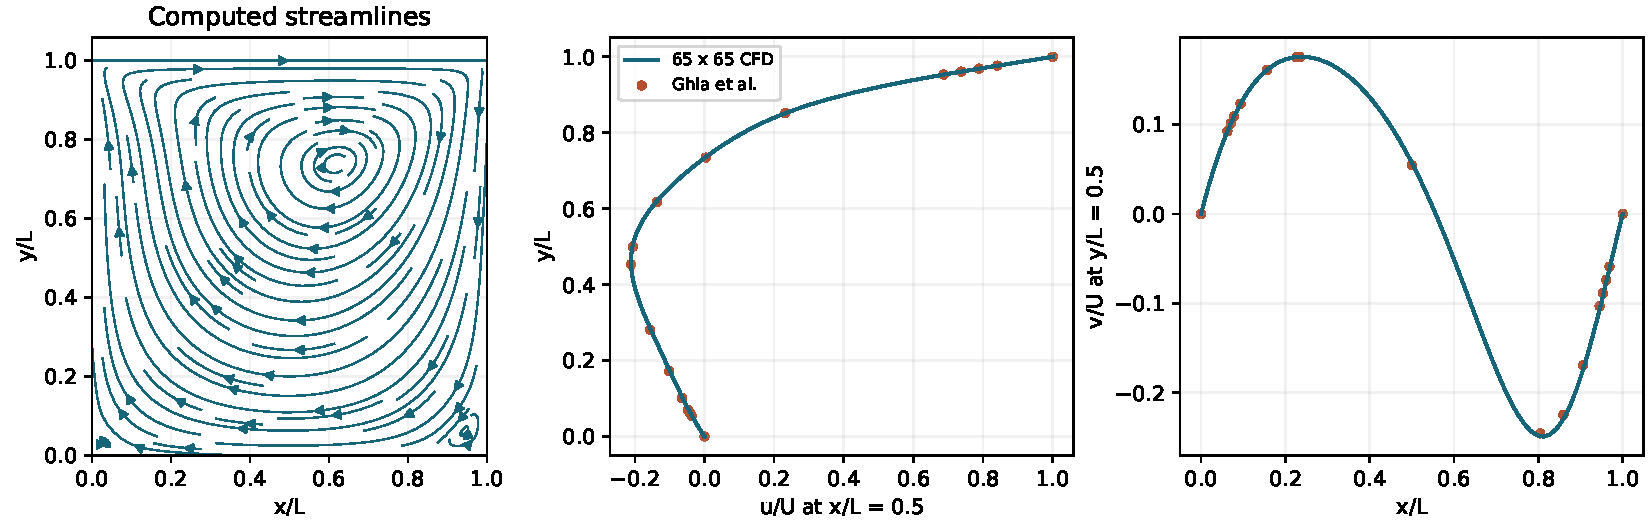
\includegraphics[width=\linewidth]{week01_assets/cavity_validation.pdf}
\end{center}
{\small\textbf{Fresh teaching computation.} Existing notebook solver, $Re=100$, $65\times65$ nodes, $\Delta t=0.001$, 10,000 steps, 60 inner sweeps per step. Markers are the notebook's Ghia table values. The relative centerline errors are $E_u=0.343\%$ and $E_v=1.771\%$; the last reported relative vorticity change is $6.02\times10^{-7}$. The associated \texttt{validation.json} records these diagnostics. This single-grid comparison is not grid-independent certification.}

\textbf{Interpret the flow.} The rightward lid drives a dominant clockwise circulation. Near the vertical centerline the lower part of the cavity has negative $u$, showing the return flow. Weak corner eddies may be difficult to resolve or display: streamline density, grid resolution, and convergence all affect their appearance. A plausible vortex alone is not validation.

\textbf{From fields to ML tensors.} A field of shape $(N_y,N_x)$ can become one channel of an array with channels $(u,v,\omega)$, and multiple cases add a batch dimension. Preserve axes, scales, boundary conventions, and parameter labels. Before using these arrays as training targets, qualify their numerical accuracy; a network trained on inaccurate CFD can reproduce its errors.
\checkpoint{Why can a visually smooth predicted vortex still have a poor centerline error or violate the wall condition?}
\newpage
\topic{12}{Optional pressure recovery and exit questions}
Taking the divergence of dimensionless momentum, using $\nabla\cdot\boldsymbol{u}=0$, gives
\begin{equation}
\boxed{\nabla^2p=-\left[u_x^2+2u_yv_x+v_y^2\right].}
\end{equation}
Under our assumptions, this is a consequence of momentum conservation, not merely an empirical approximation. For dimensional pressure the right-hand side carries a factor $\rho$ and uses dimensional velocity gradients.

\textbf{The right-hand side is not the whole pressure problem.} Boundary conditions must also be supplied consistently with momentum. For outward wall normal $\boldsymbol{n}$,
\begin{equation}
\frac{\partial p}{\partial n}=\boldsymbol{n}\cdot\left[-\partial_t\boldsymbol{u}-(\boldsymbol{u}\cdot\nabla)\boldsymbol{u}+Re^{-1}\nabla^2\boldsymbol{u}\right].
\end{equation}
One must handle discrete compatibility when using Neumann data. Pressure is then determined only up to an additive constant: set a reference value or subtract its mean. Subtracting the mean fixes the gauge; it does not repair an incorrect pressure boundary condition. Pressure reconstruction is an extension, not a prerequisite for the Week-1 velocity solve.

\textbf{After Week 1, you should be able to}
\begin{enumerate}
\item Write continuity and both momentum components, and derive their nondimensional form.
\item Define $\psi$ and $\omega$, explain their physical meaning, and prove $\nabla^2\psi=-\omega$.
\item Explain why the vorticity equation needs velocities and how the coupled solve obtains them.
\item Convert a derivative and the Poisson equation into finite differences, keeping array axes consistent.
\item Distinguish inner Poisson iteration, outer time evolution, stability, convergence, and validation.
\item Compare centerline profiles quantitatively and describe the limits of that evidence.
\end{enumerate}
\textbf{Optional derivation exercise.} Reproduce the curl-of-momentum calculation on page~7, identifying the exact use of incompressibility. Then derive the moving-wall vorticity formula from a Taylor expansion.

\textbf{References and authorship scope}
\begin{enumerate}[label={[\arabic*]}]
\item U. Ghia, K. N. Ghia, and C. T. Shin (1982). High-Re solutions for incompressible flow using the Navier--Stokes equations and a multigrid method. \emph{Journal of Computational Physics}, 48, 387--411. Benchmark data used by the existing notebook.
\item F. M. White and H. Xue (2022). \emph{Fluid Mechanics}, 9th ed. McGraw Hill. Background on conservation laws and incompressible flow.
\item J. D. Anderson (1995). \emph{Computational Fluid Dynamics: The Basics with Applications}. McGraw Hill. Background on discretization and numerical solution.
\end{enumerate}
{\small Explanations and derivations were independently written for FlowMLLab's introductory cavity example, using the requested topic checklist. The figure is a fresh execution of FlowMLLab's own solver. No restricted course text, solution, figure, or code was incorporated. No ML split or calibration is involved in this numerical-foundations extension; its baseline is the stated Ghia centerline comparison.}
\end{document}
